\documentclass[a4 paper,11pt,2]{article}

%les packages utilisés habituellement, permettent de tout faire grosso modo

\usepackage{amsfonts}
\usepackage{amsmath}
\usepackage{amssymb}
\usepackage[utf8]{inputenc}
\usepackage[french]{babel}
\usepackage{lmodern}
\usepackage{pdflscape}

\usepackage{stmaryrd}
\usepackage[T1]{fontenc}
\usepackage{xcolor}
\usepackage{mathrsfs}
\usepackage{enumitem}
\usepackage{helvet}
\usepackage{indentfirst}

\usepackage{graphicx}
\usepackage{subfig}
\usepackage{setspace}
\usepackage{fancyhdr}
\usepackage{tikz-cd}
\usetikzlibrary{shadows,shapes,positioning,bending}
\usepackage[ruled]{algorithm2e}

\usepackage{hyperref}
\usepackage{biblatex}

\newcommand{\HRule}{\rule{\linewidth}{0.5mm}}
\newcommand{\dpart}[2]{\frac{\partial #1}{\partial #2}}
\newcommand{\scal}[2]{\langle #1,#2 \rangle}
\newcommand{\Four}[2]{\mathcal{F}\left\{#1\right\}(#2)}
\newcommand{\Z}{\mathbb{Z}}
\newcommand{\indic}{1\!\!1}

\newtheorem{prop}{Proposition}
\newtheorem{theorem}{Théorème}
\newtheorem{defin}{Définition}

\DeclareMathOperator*{\argmax}{arg\!\,max}
\DeclareMathOperator*{\argmin}{arg\!\,min}
\DeclareMathOperator*{\minimize}{mini\!\,mize}
\DeclareMathOperator*{\maximize}{maxi\!\,mize}

\setlength{\hoffset}{-18pt}
\setlength{\oddsidemargin}{0pt} % Marge gauche sur pages impaires
\setlength{\evensidemargin}{9pt} % Marge gauche sur pages paires
\setlength{\marginparwidth}{54pt} % Largeur de note dans la marge
\setlength{\textwidth}{481pt} % Largeur de la zone de texte (17cm)
\setlength{\voffset}{-18pt} % Bon pour DOS
\setlength{\marginparsep}{7pt} % Séparation de la marge
\setlength{\topmargin}{0pt} % Pas de marge en haut
\setlength{\headheight}{13pt} % Haut de page
\setlength{\headsep}{10pt} % Entre le haut de page et le texte
\setlength{\footskip}{27pt} % Bas de page + séparation
\setlength{\textheight}{708pt} % Hauteur de la zone de texte (25cm)

\pagestyle{fancy}
\fancyhead[L]{\leftmark} % Positionne le numéro de chapitre dans le coin en haut à gauche
\fancyhead[R]{} % Rien dans l'en-tête à droite
\fancyfoot[L]{CentraleSupélec} % Le nom de ton école préférée dans le pied de page gauche
\fancyfoot[R]{ICE P2024} % Ta promo dans le pied de page droit
\renewcommand{\footrulewidth}{0.5pt} % Largeur du trait de séparation dans le pied de page

\hypersetup{hidelinks=true}
\addbibresource{biblio.bib}

\begin{document}
\begin{titlepage}
\begin{center}

% Upper part of the page. The '~' is needed because only works if a paragraph has started.

\includegraphics[width=\textwidth]{./logo}~\\[1cm]

%\textsc{\LARGE Université ou Entreprise}\\[1.5cm]

\textsc{\Large }\\[0.5cm]

% Title
\HRule \\[0.4cm]

{\huge \bfseries Deep Learning Project Report\\
[0.4cm] }

{\large \bfseries Quentin Goulas, Lucas Hocquette\\[0.4cm] }
%{\large \bfseries \textit{}\\ }
{\large \bfseries \textit{ICE P24}\\[0.4cm] }


\HRule \\[1.5cm]

\vspace{3cm}

% Author and supervisor
%\begin{minipage}{0.4\textwidth}
%\begin{flushleft} \large
%\emph{Réalisé par le groupe no. \ldots :}\\
%	Prénom \textsc{Nom} \\
%	Prénom \textsc{Nom} \\
%	Prénom \textsc{Nom}
%\end{flushleft}
%
%\end{minipage}


\vfill

% Bottom of the page
{\large December - 2024}

\end{center}
\end{titlepage}

%\thispagestyle{empty}
\tableofcontents
\newpage

This project report aims to present the development framework, methodology and
results obtained during the Deep Learning course project. This project focussed
on hyperparameter optimization methods for deep learning models.

This report comprises four sections : an introduction to the project its
premises, a presentation of the considered algorithms for this project, a
description of the deployed system architecture and finall a discussion on the
obtained results.

\section{Project introduction}
In the context of deep learning, hyperparameters are model parameters that
aren't learnt by the model yet impact the learning capacity of the model.
Hyperparameters include, but are not limited to :
\begin{itemize}
    \item model architecture : number of hidden layers, size of the hidden layers, layer
          type (dense, convolutional, recurrent, ...), activation function of the layer
    \item preprocessing : normalization, data augmentation, ...
    \item regularization : Lasso, Tykhonov, dropout layers, ...
    \item loss function choice : euclidean distance, cross-entropy loss, ...
\end{itemize}

The choice of good hyperparameters is crucial to have a well-functioning model
where having too simple a model may induce underfitting whilst building too
complex a model might lead to overfitting. Yet, choosing the appropriate
hyperparameters implies training an important number of models with different
hyperparameters configuration, which induces high computing costs. Finding
efficient methods to obtain the optimal hyperparameter configuration for a
given DL task is therefore a topic of choice for the deep learning literature.

The most used Hyper Parameter Optimization (HPO) methods include \cite{yangHyperparameterOptimizationMachine2020} :
\begin{itemize}
    \item Babysitting : try different hyperparameter configurations, assess the accuracy
          of the different models, manually adjust the configurations and repeat till
          convergence. This method can be computationnaly intensive and labor intensive
    \item Grid search : try all the possible hyperparameter configurations and select the
          best one. This method requires very important computational and time resources,
          as well as a discrete hyperparameter space to evaluate
    \item Random search : try a proportion of randomly chosen hyperparameters in the
          possible hyperparameter space and select the best performing configuration
          among the tested configuration
    \item Gradient-based optimization : uses a gradient-descent approach to find the next
          hyperparameter configuration to evaluate. This requires a loss function that is
          differentiable in the hyperparameter variables
    \item Particle Swarm Optimization (PSO) : uses the particle swarm optimization
          algorithm to find the optimum fo a given function
    \item Genetic Algorithms which uses the genetic heuristic to find the optimal
          hyperparameters
    \item Bayesian methods using a modelled prior on the model loss function to converge
          to the best hyperparameter configuration
\end{itemize}

This project aims at implementing a HyperParameter Optimization framework to
compare different hyperparameter optimizers. For this project, we will focus on
Grid Search, Random Search, Bayesian Optimizer Hyper Band and Particle Swarm Optimization (said to be the best
hyperparameter optimizing method in the current literature)

\section{Algorithm descriptions}
We describe here the algorithms that have been implemented throughout this
project : Grid search, Random search, Particle swarm optimization. We also provide the pseudo-codes for the methods.

\subsection{Grid search}
This method consists in ``brute forcing'' the best hyperparameter configuration, i.e by trying all possible hyperparameter configurations on the hyperparameter space and returning the best configuration. This method is extremely computationnaly heavy, with the number of possible configurations increasing exponentially as the number of tested hyperparameters increases.
\begin{algorithm}
    \SetAlgoLined
    \KwIn{Hyperparameter space $H$, training set $D$, validation set $V$}
    \KwOut{Best hyperparameter configuration $h^*$ and accuracy $a^*$}
    \For{each hyperparameter configuration $h$ in $H$}{
        Train model $M$ with hyperparameters $h$ on $D$\;
        Evaluate model $M$ on $V$ and compute accuracy $a$\;
        \If{$a > a^*$}{
            $h^* \leftarrow h$\;
            $a^* \leftarrow a$\;
        }
    }
    \Return{$h^* , a^*$}
    \caption{Grid search algorithm}
\end{algorithm}

\subsection{Random search}
This method consists in randomly selecting a proportion of all the possible hyperparameter configurations and returning the best configuration after trying all configurations in the sample. This method reduces slightly the computational time compared to grid search. However, this method does not solve the curse of dimensionality problem. As a matter of fact, the only method to solve this problem is to use a sampling proportion of the order $p^d$ with the $d$ the number of hyperparameters. This technique keeps computation time constant but dramatically reduces the exhaustivity of the method and success probability of the algorithm.
\begin{algorithm}
    \SetAlgoLined
    \KwIn{Hyperparameter space $H$, training set $D$, validation set $V$, sampling proportion p}
    \KwOut{Best hyperparameter configuration $h^*$ and accuracy $a^*$}
    \For{each hyperparameter configuration $h$ in $H$}{
    	$r\sim \mathcal{U}([0,1])$\;
        \If{random number $r < p$}{
            Train model $M$ with hyperparameters $h$ on $D$\;
            Evaluate model $M$ on $V$ and compute accuracy $a$\;
            \If{$a > a^*$}{
                $h^* \leftarrow h$\;
                $a^* \leftarrow a$\;
            }
        }
    }
    \Return{$h^* , a^*$}
    \caption{Random search algorithm}
\end{algorithm}

\subsection{Particle Swarm Optimization}
The particle swarm optimization algorithm is a metaheuristic optimization algorithm which assumes next to no information on the functions to optimize. Modelled on the evolution of bird flocks, it consists in evaluation the model accuracy on a small set of hyperparameter configurations, then choosing a new set of configurations on the basis of the best configuration seen overall and by the best configuration seen by the particles individually.

\begin{algorithm}[H]
    \SetAlgoLined
    \caption{Particle Swarm Optimization (PSO) algorithm}
    \KwIn{Hyperparameter space $H$, training set $D$, validation set $V$, swarm size $S$, $\phi_l$ local step size, $\phi_g$ global step size, $w$ inertia, precision $\epsilon$}
    \KwOut{Best hyperparameter configuration $h^*$ and accuracy $a^*$}
    \BlankLine
    Initialize the personal best position vector $\mathbf{p}_0$ to $\mathbf{x}_0$\;
    Initialize the position vector (randomly taken from $H$) $\mathbf{x}_0$ of the swarm\;
    Initialize the speed vector $\mathbf{v}_0$ to $\mathbf{0}$\;
    Initialize and compute accuracy vector $\mathbf{a}_0$ of the swarm $\mathbf{x}_0$\;
    $t \leftarrow 0$\;
    $ a^* , h^* \leftarrow \max(\mathbf{a}_0), \mathbf{x}_0[\argmax(\mathbf{a}_0)]$\;
    \BlankLine
    \Repeat{$\left\lVert \mathbf{v}_t \right\rVert < \epsilon$}{
    Compute $\mathbf{a}_t$ of the swarm $\mathbf{x}_t$\;
    $\tilde{a}, \tilde{h} \leftarrow \max(\mathbf{a}_t), \mathbf{x}_t[\argmax(\mathbf{a}_t)]$\;
    \If{$\tilde{a} > a^*$}{
        $a^* , h^* \leftarrow \tilde{a}, \tilde{h}$\;
    }
    $t \leftarrow t+1$\;
    Take $u_l$ and $u_g$ uniformly from $[0,\phi_l]$ and $[0,\phi_g]$\;
    $\mathbf{v}_t \leftarrow \mathbf{v}_{t-1}.w + (\tilde{h} - \mathbf{x}_{t-1}).u_l + (h^* - \mathbf{x}_{t-1}).u_g$\;
    $\mathbf{x}_t \leftarrow \mathbf{x}_{t-1} + \mathbf{v}_{t}$\;
    }
    \BlankLine
    \Return{$h^*, a^*, t$}
\end{algorithm}

The convergence of the Particle Swarm Optimization algorithm cannot be proven in the general case (although some refinements can provide convergence to a local optimum \cite{engelbrechtConvergenceProofParticle2010}). Yet, empirical data shows the efficiency of this algorithm in a majority of cases.

\subsection{Bayesian Optimization HyperBand algorithm \cite{falknerBOHBRobustEfficient2018}}
This method uses a probabilistic model of the accuracy function given the different tested configurations and iteratively returns the next configuration to try out by choosing the maximizer of expected improvement.  The probabilistic model used here is the Tree Parzen Estimator which uses a kernel density estimator to model the accuracy function of the model. To further improve the performance of the algorithm, the Hyper Band technique is used to dynamically allocate the amount of resources for each training. For this project, we rely on the \href{https://automl.github.io/HpBandSter/build/html/quickstart.html}{HpBandSter library [clickable link]} which provides a full BOHB optimizer framework ---similar to ours--- that we integrated to our framework. Furthermore, this library enables asynchronous processing to try out multiple configurations simultaneously, therefore drastically increasing computing efficiency.

\section{Development framework}
This project will be entirely developed on Python through the Pytorch deep
learning library. Moreover, the CIFAR-10 dataset will be used throughout this
study to train a LeNet5-type model architecture for image recognition. Our
hyperparameters of interest are the output sizes of the
convolutional layers (C1, C3, C5) and the output size of the first dense layer (F6)

For this project, we decide to build a HyperParameterOptimizer (HPO) object
responsible for navigating the input hyperparameter space and organizing the
different hyperparameter configuration tests. The HPO object then calls a
dedicated library to generate a model with the appropriate hyperparameters and
launches the trainings. The system architecture is given in Figure
\ref{fig:framework}.

The accuracy function of the classifier is chosen as the proportion of accurate classifications from the model on a validation dataset.

\begin{figure}[h]
    \centering
    \begin{tikzpicture}
        \draw (-3.33,7.25) node(input) [draw]{\begin{tabular}{c} Data, Seed,\\ Method,\\ Method parameters\end{tabular}};
        \node[matrix, draw, column sep =0cm, inner sep = 0.75cm, rounded corners =4pt] (hpo) at (1,4)
        {
            \node[rectangle, draw] (object) at (0,0) {\begin{tabular}{c}Hyper Parameter\\ Optimizer\end{tabular}}; & \node at (0.5,0) {\small{$\circlearrowright$ Iterate till convergence}}; & \node[rectangle, draw] (model) at (1,0) {DL Model};\\
        };
        \draw (-3.33,1) node(output) [draw] {\begin{tabular}{c}Best Hyperparameter\\ configuration\end{tabular}};
        \draw [anchor=east](7.5,2) node(comment) [fill=white] {Hyper parameter optimization framework};
        \draw [-Latex] (input.south) -- node[below left] {\small{Inputs}} (object.north);
        \draw [-Latex] (object.south) -- node[above left]{\small{Outputs}} (output.north);
        \draw [-Latex] ([yshift=5pt]object.east) to[bend left] node[above] {\small{\begin{tabular}{c}Hyperparameter\\ configuration\end{tabular}}} ([yshift=5pt]model.west);
        \draw [-Latex] ([yshift=-5pt]model.west) to[bend left] node[below] {\small{Model accuracy}} ([yshift=-5pt]object.east);
        \draw [-Latex, rounded corners=4pt] (model.north) |- node[above] {train\_model} (8.1,5.25) |- (model.east);

    \end{tikzpicture}
    \caption{Hyper parameter optimization workflow}
    \label{fig:framework}
\end{figure}

To improve scalability, hyperparameter configurations are parsed as
dictionaries, with name-value pairs of hyperparameter name and corresponding
values. This enables to manipulate the same objects across hyperparameter
spaces (which are hyperparameter configurations with multiple accessible
values) and hyperparameter arrays (used to represent multiple hyperparameter
configurations simultaneously).

\section{Experimental setup}
To try out the different hyperparameter optimizers, we search for the optimal configurations of a LeNet-5 type network \cite{lecunGradientbasedLearningApplied1998}. More precisely, we look for the optimal number of filters for the three convolutional layers C1, C3 and C5 as well as the size of the network's dense layer F6. A schematic of the LeNet-5 architecture is provided in Figure \ref{fig:lenet}.

\begin{figure}[h]
\centering
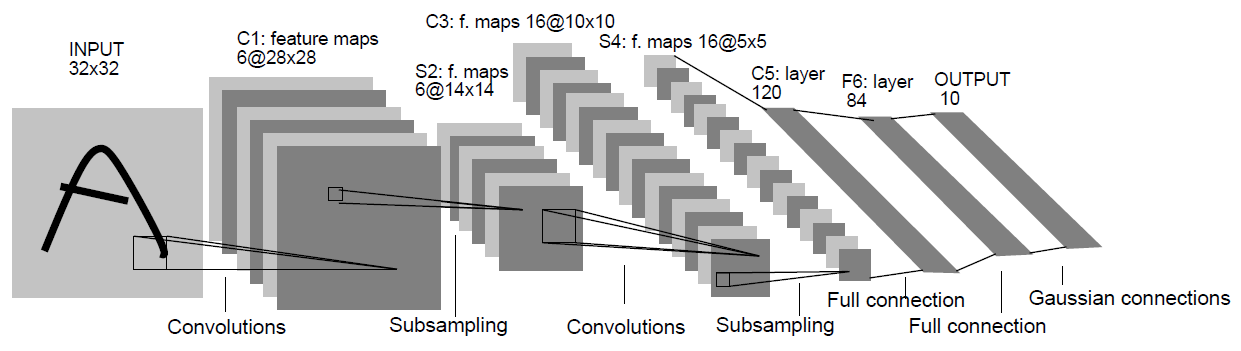
\includegraphics[width = \linewidth]{ln5.png}
\caption{LeNet-5 architecure with the hyperparameter configuration used in the original paper}
\label{fig:lenet}
\end{figure}

We use the LeNet-5 architecture to recognize different images from the CIFAR-10 dataset \cite{krizhevskyLearningMultiplyeLayers2009}, divided into 10 categories : \{ airplane, automobile, bird, cat, deer, dog, frog, horse, ship, truck\}. The CIFAR-10 comprises $60\ 000$ coloured images of $32\times32$ pixels with $6\ 000$ images per category and split into a $50\ 000$ image training set and a $10\ 000$ image test set.

Model trainings for this project have been entirely done on local GPUs (GeForce MX230 and GeForce RTX3070 Laptop) with a batch of size 64. Training the classifier on CIFAR-10 as provided by \verb+torchvision+ led to an epoch duration from 20 to 40s depending on model complexity.

We use the following parameters for each algorithm :
\begin{figure}[h]
\centering
\begin{tabular}{|c|c|}
\hline Algorithm & Parameters \\
\hline Grid search & $\emptyset$ \\
Random search & p = 0.5 \\
Particle Swarm Optimization & $S=5,\phi_l = 2,\ \phi_g = 2,\ w=0.5$\\ \hline
\end{tabular}
\label{tab:parameters}
\caption{Algorithm parameters}
\end{figure}

Unless indicated otherwise, the number of epochs for every trainings is set at 40.

Although the implemented algorithms enable increased efficiency compared to a babysitting or grid search approach, each optimization run took considerable amounts of time, allowing minimal repetitions to validate the results, leaving significant space to interpretation of the results and little quantitative results. We still present the results in the following section.

\section{Results}

Running the algorithms returns us the following results :
\begin{figure}[h]
\centering
\begin{tabular}{|c|c|c|}
\hline Algorithm & \begin{tabular}{c}Hyperparameter config\\ \hline \begin{tabular}{c|c|c|c}F6&C1&C3&C5\end{tabular}\end{tabular} & Number of training epochs \\
\hline Particle Swarm Optimization & $\cdots$ & $\cdots$\\ \hline
\end{tabular}
\label{tab:results}
\caption{Optimal hyperparameter configurations}
\end{figure}

Due to the extreme resource consumption of grid search, we weren't able to do a run for this algorithm.

\addcontentsline{toc}{section}{References}
\printbibliography

\end{document}